% TODO 
% discuss fig 4 
% not refere to skyline whith angleshizzle because this is the first time
% be more clear about the projection, its the first time the reader sees it 


%TODO general advise
% motivate my assumption and choices 
% explain stepwise if the reader is dumb
% can en could niet in dezelfde zin gebruiken, zelfde tijd gebruiken
% zoeken op 'but' en kijken of er however bij kan


%TODO2 (is a categorie of would be nice TODO's)
%
% zoeken of Figure en dan labels and refs gebruiken
% zoeken of chapter en dan labels and refs gebruiken
% aan alle eind alinea \\ zetten
% fill caption of figures
% search what houghline (and canny edge for report.tex) params I used

% TODO
% discussion:
% Furthermore it would be good to fully discard the flat roof assumption. This will allow a building to have any shape, which is nice. The drawback is that a new method of outlier detection has to be developed. 
% Object recognition play a great part in this. If one knows where, for example, an occluding object is located, this could be used to filter the output of the skyline detector. This however rises a new problem, namely that the 3D model has no augmentations at the position of occluding objects. Determining what would be located behind the occluding object would be an interesting AI challenge and will incorporate pattern recognition, making use of repetitive structures and off course combining the multiple views to reveal as much information as possible.\\


%TODO aan het eind
% read again and check level of detail, is it everywhere the same?
% do I do enough chaining?
% read again on other subjects in mind see how te wr thesis
% spell check!!

% TODO IDEEEN
% polygonal models fitten bij dakkapels

\section{Improving the 3D building}
\subsection{Introduction}
%chain
In the previous chapter we extracted the building contour with the skyline
detector. The output was a set of 2D points and we collected this set for every
view of the building.  The aim of this chapter is to use this set of points to
improve a basic 3D model. \\
The point cloud from the skyline detector included a lot of noise caused mostly
by occluding objects like trees. How do we detect those outliers?
And if we have an outlier free point cloud how can we use this information to
improve a basic 3D model? And how do we know which point is associated to which part of the
building?  These questions are addressed in this chapter.\\
We present a stepwise solution. First \emph{Openstreetmap} is used to generate
a basic 3D model of a building. Secondly the set of points returned by the
skyline detector is transfered to a set of lines. Then each line segment is
assigned to a wall of the building. After this the lines are projected to these
assigned walls in the 3D model.  The projections are used to estimate new
height values of the building walls.  The 3D model is finally improved by updating the
walls according these heights. \\
We will now elaborate on each step.\\

\subsection{Generating the 3D model}
The 3D model is generated using a basis (groundplane) which is manually extended.
The basis (viewed from top) of the generated 3D model is originated from
\emph{Openstreetmap}.\\
\fig{openstreetmap}{}{0.25}
Openstreetmap, see Figure 1,is a freely accessible 2D map generated by
users all over the world. It contains information about streets, building
contours, building functions, museums, etc.  We are interested in the building
contours.  We take a snapshot of one particular area and extract this building
contour.  This is a set of ordered points where each point corresponds to a
corner of the building.  Next we link these points to walls.\\ 
Because the map is based on aerial images, it is in 2D and contains no
information regarding the height of each wall.  \\
The final 3D model is generated by starting with the the 2D building contour as
its basis. We estimate the wall heights by hand and overestimate this height.
After this we use the height to extend the 2D basis in the opposite gravity direction,
resulting in a 3D model.\\\\
\textbf{\emph{Gravity aligned walls assumption}}\\
	\emph{The walls of the building are aligned in the opposite direction of the gravity
	which is orthogonal to the 2D basis from \textbf{Openstreetmap}}.\\

% Extending the 2D basis with a finite height is only for illustration purposes, the algorithm
% actually works with infinite high walls. 
% This is done to make sure we don't miss
% a , more on this in section 
An example of the 3D model can be seen in Figure 4.

% why not ransac?
\subsection{Extracting line segments}
%intro
	The skyline detector returned a set of points. If some of these points lie
	on the same line, they form a straight line.  Straight lines are likely to
	come from the building contour. If we have a method that extracts these
	straight line segments, we can use these line segments to find parts of the
	building contour and finally use this to improve the 3D model.\\
	Unfortunately a problem arises because some points are outliers. To discard these outliers
	we detect the inliers and consider the remainder as outliers.  In this
	section we draw an assumption and we explain how straight line segments are extracted and how
	outliers are discarded at the same time.\\


	\paragraph{Assuming a flat roof}
	Many urban areas contain buildings with a flat roof. This means that the
	contour of the building is mostly formed by straight lines.  We use this
	fact to simplify our problem:\\\\
	\textbf{\emph{Flat roof assumption}}\\
	\emph{We assume each building has a flat roof, implicating that each building wall
	has a straight upper contour. The walls may have different heights but the roof should be flat.}\\

	This assumption is very useful as it let us focus on finding the height
	of the building walls from the building contour without having to concern
	for (complex) rooftypes.  This doesn't mean that the method described in
		this thesis is unusable for buildings that contain roofs. E.g.
		with a small adjustment the method could be used to at least
		gain the building height which is a useful application.\\
	Ideas about how to handle rooftypes explicitly can be found in the
	Future work section.\\

\subsubsection{Hough transform}
	A widely used method for extracting line segments is the Hough transform \cite{Hough}
	We regard this as a suitable method because it is
	used a lot for this kind of problems. This is probably because it is unique
	in its low complexity (compared to other (iterative) methods like
	\emph{RANSAC}).\\
	% TODO motivate why not ransac, search for papers about line segments,
	% reference them
	In the Hough transform, the main idea is to consider the characteristics of a
	straight line not as its image points $(x1, y1)$, $(x2, y2)$, etc., but in
	terms of the parameters of the straight line formula $y = mx + b$. i.e., the
	slope parameter $m$ and the intercept parameter $b$.\\
	The input of a Hough transform is a binary image, in our case the output of 
	the skyline detector (chapter ?).\\
	If a pixel is classified as a skyline pixel (a pixel that lies on the
	skyline according the skyline detector), the Hough transform increases
	a vote value for every valid line ($m$,$b$ pair) that crosses this
	particular pixel.  Lines ($m$, $b$ pairs) that receive a large amount of votes
	contain a large amount of skyline pixels.\\
	Because the algorithm detects straight lines containing only skyline pixels it is
	most likely that it returns parts of the skyline and therefore the building
	contour. \\ The Hough transform is implemented in \emph{Matlab} and has
	some useful extra functions.The algorithm can optionally return the start
	and endpoint of the found lines which is very useful as it helps us to
	associate which part of the building is described by the line.\\
	Furthermore it has the parameter \emph{FillGap} that specifies the distance
	between two line segments associated with the same $m$,$b$ pair.  When this
	inter line segment distance is less then the \emph{FillGap} parameter, it
	merges the line segments into a single line segment. In our application
	this parameter is of particular interest when we want to merge lines that
	are interrupted by for example an occluding tree.\\
	Results of the Hough transform on the 2D output of the skyline detector are
	displayed and evaluated in the Result section.



\subsection{Project the skyline to the building}
%TODO name different methods? and put in table and test
% Some different methods
% method 1:
% take endpoints and project, con: endpoints don't agree
% see above tekst
% method 2:
% middle point
% method 3: 
% overlap

	% intro
	The Hough transform of the previous section returned a set of 2D line
	segments which present parts of the skyline.  If we can find a way to
	project these lines to the building we can improve our basic 3D model.
	
	This involves three steps, the calibration of the camera,
	the projection to the building and a way to
	associate a skylinepart with a specific buildingpart.
	% TODO organisation of chapter uitleggen of niet?
	% First, a few assumption are made and the details of the problem are
	% analyzed. Secondly the developed method of projection and line-wall
	% association is explained.\\
	%TODO POLIJSTEN

	%TODO intronize projection
	%TODO how does the 3d model helps us?

	\subsubsection{Camera calibration}

	\paragraph{Extrinsic parameters}
	
	%\paragraph{Getting the camera centers and viewing directions}
	%TODO introduce viewing direction
	How do we find the the camera centers (positions) and camera viewing
	directions. In some systems this is known on forehand by measuring the cameras position and
	orientation at the scene. In other systems, as in ours, this is calculated 
	afterwards.  We calculated the values afterwards and used the
	\emph{Fit3d toolbox} \cite{Fit3d} for this.
	 See preliminaries (%TODO
	) for detail.\\  
	%TODO uitleggen hoe (fit3d toolbox)

	\paragraph{Intrinsic parameters}
	%\paragraph{Getting the calibration matrix}
	%TODO inspriation
	% isaacs paper 
	% google 
	% matlab help bouget 
	%

	% %TODO
	% "relationship between what appears on the image (or retinal) plane and where
	% it is located in the 3D world."
	% intrinsic 
	% extrinsic params

	As it is our own dataset we also know what camera took the picture so we can
	calculate a camera specific Calibration matrix.  
	%TODO explain rotation, translation
	%TODO intrinsic extrinsic parametrs
	The calibration matrix is retrieved by making images of a chessboard in
	different positions and orientations together with the Bouget toolbox.
	More on this in the preliminaries.
	 
	\subsubsection{From image point (2D) to possible points in scene (3D)} 
	The line segment that was returned by the Hough transform consists of two
	endpoints $v$ and $w$. These endpoints are in 2D but are recorded in a 3D
	scene and therefor present a 3D point in space.  The value of the 3rd
	dimension represents the distance from the 3D point to the camera that took
	the picture. Unfortunately this value is unknown, however because we
	calibrated the camera we can reduce the possible points in 3D space to a
	line.\\
	See Figure %TODO make figure of line that goes into scene

	We know:
	\begin{itemize}
		\item The 2D properties about the pixel, (the location of the pixel in the image). 
		\item The camera's internal parameters (Calibration matrix) \\
		\item The translation of the camera
		\item The rotation of the camera
	\end{itemize}

	We can now define the line of possible points in 3D space by two coordinates:\\
	\begin{itemize}
		\item $C$, the center of the camera, and
		%TODO %(camera centers are annotated for every image)
		\item $K'p$, the point that lies on the retina of the camera, where $K$ is the Calibration matrix and $p$ is the homogeneous pixel coordinate.
		%TODO explain Why K'p
		%TODO add P
	\end{itemize}
	%TODO image

	%TODO zee zisserman pagenumbers in feedbackmap
	%TODO REF over hoe je van 2 coords naar een lijn gaat

	%So the problem is boiled down in finding the Camera centers and viewing
	%directions and finding the
	%Calibration matrix.\\

	Now we have the two required coordinates, we can set up an equation of the
	line of possible points in 3D.
	This is done as described in preliminaries (Transform coordinates to a line equation). 

	\subsubsection{Intersecting with walls}
	%TODO write in intro 
	%For every line segment we now have two endpoints which are transformed to an
	%infinite line of possible points in the scene.  We are now ... your friend 
	%TODO larger intro
	%To know which linesegment presents which wall we are intersecting the infinite
	%lines with the walls. 
	%
	%The building is first divided into different walls.  Every wall of the building spans a plane. 
	%Intersections are then calculated between the lines and the planes of the building walls.\\


	As described in %TODO
	 the 3D building model is divided into different walls. These walls are
	 described by two ground coordinates and a direction which is the y-direction as
	 assumed by the \emph{Gravity aligned walls assumption}.

	As you can read in preliminaries (Planes and walls) the walls are transformed
	into planes.  This is done for two reasons: first this transformation is required to calculate the intersection properly.
	Secondly, because the 3D model is an estimate, the walls maybe just
	to small which could %TODO ongewenst
	result in no intersection which is unwanted.
	%TODO example image

	Now we have the building divided op into planes we can intersect the lines.
	%TODO intersection formula 
	%TODO 
	%Note that
	%A skyline pixel intersects with every wall as both the lines and planes are
	%infinite and have a very low change of being parallel.

	For every line segment we have two endpoints which are now projected on the
	building walls
	This results in 2xlxw points in 3D, grouped by the line segments, where $l$ is the number
	of lines and $w$ is the number of walls. 

	The next challenge is to reduce the number of intersection for every line
	segment to one. In other words, to determine the wall that is responsible for
	the line segment. This is later on used to update the height of the wall of the
	3D model.\\


\subsubsection{Associating line segments with building walls}
%TODO intro
	\paragraph{Assumptions}
	We consider each building consisting of seperate walls and associate each
	line segment with a wall of the building that is most likely responsible for
	that line segment. \\
		
	%TODO2 numbered assumptions
	\textbf{	\emph{Unique wall assumption:}}\\
	\emph{We assume that the output of the Hough transform are line segments
	that each represent a single wall of the building, e.g. if the Hough
	transform finds 3 line segments there are 3 walls present.}\\

	\textbf{	\emph{Building wall appearence assumption:}}\\
	\emph{We assume that every line segment in the output of the Hough transform represent (a part of) the upper side of
	a specific wall of the building.}

	If a line segment is assumed to represent a single wall then the projection
	to that wall should have a large overlap with this wall.  To be more
	precise, let's define $l$ in $\mathbb{R}2$ as a line segment that is
	generated by the Hough transform.  If we project $l$ to the plane spanned
	by a wall $W$ we get a line $l_{proj_W}$ in $\mathbb{R}3$.  If we assume
	$l$ to come from contour of wall $W$, then $l_{proj_W}$ should have a large
	intersection with this wall $W$ (as we overestimated the height of the
	building). We call this the line-wall overlap value, $lwo$.  A mathematical
	definition of $lwo$ follows.  Note that the projection of $l$ with the
	other walls should have a small $lwo$ value.
	%TODO2. see figure, create two Figure's (2d and 3d) with a single houghline
	%(projected)

	\textbf{	\emph{Largest line-wall overlap assumption:}}\\
	\emph{A line segment describes the contour of the wall where its projection
	has the largest overlap with.}\\

	%\subsubsection{Line-wall association}
	Having defined the assumptions, the situation and the idea behind the
	line-wall association, we can now explain the line-wall matching algorithm.\\ 

	A line segment is projected to all walls and the amount of line-wall
	overlap, $lwo$ is calculated. The wall with the largest overlap with the specific line
segment is classified as the most likely wall for that line segment.
	Next the line segments are projected to their most likely wall and the
	algorithm outputs this set of lines in $\mathbb{R}3$. 
	

	%\paragraph{Line wall overlap type}
	This line-wall overlap is calculated in different steps.
	First, different types of overlap are explained. Secondly the algorithm
	determines the \emph{overlap type}, then the overlap amount is determined and
	finally the amount of overlap is normalized.\\

	$l_{proj_W}$ can overlap $W$ in four different scenarios, this is explained
	in Figure 10. The wall $W$ is spanned by $abcd$, and $l_{proj_W}$ is spanned
	by $vw$.
	

	% fig only works with pdflatex, hmmz, but then fig nr's don't work

	% \begin{figure}[!ht]
	% \centering
	% 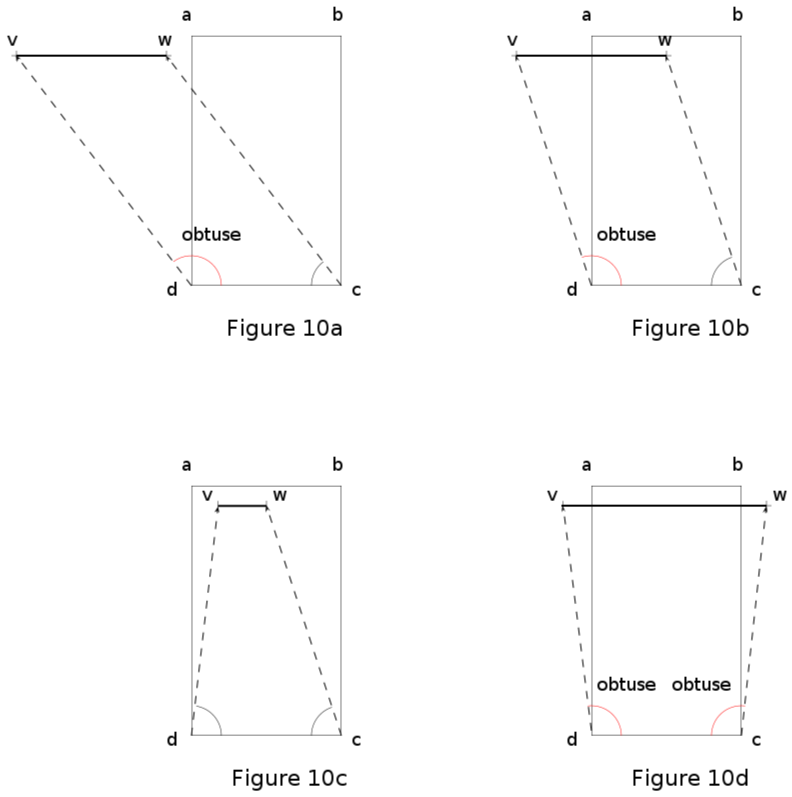
\includegraphics[width=12cm]{img/overlaytypes.png}
	% \end{figure}
		
	\fig{overlaytypes}{}{0.4}

% captions of the Figure
%		1) no overlap (see fig 10a)\\
%		2) partial overlap (fig 10b)\\
%		3) full overlap ($l_{proj_w}$ is included in $w$)(fig 10c)\\
%		4) full overlap ($l_{proj_w}$ overextends $w$) (fig 10d)\\

	The type of overlap is defined by exposing the endpoints of the line
	segments to an \emph{in polygon} test, where the polygon represents a 
	wall of the building (e.g. $abcd$ in Figure 10).
	%TODO REF MATLAB?
	%we use the Matlab build in polygon as in section (%TODO)

	The table below represents the types of overlap with the corresponding number of points
	that pass the \emph{in polygon} test and their possible line-wall overlap
	value.\\ 

	\begin{tabular}{|l||c|c|c|}
	\hline
	Type of line-wall overlap 			&	Points in polygon 			& Line-wall overlap & Figure \\
	\hline
	\hline
	No overlap					&	0					& 0		& 10a\\
	\hline
	Partial overlap 				&	1					& [0..1]	& 10b\\
	\hline
	Full overlap (included)		&	2					& 1		& 10c\\
	\hline
	Full overlap (overextended)		&  	0					& 1 		& 10d\\
	\hline
	\end{tabular}

	\paragraph{No overlap}
	If the point in polygon test returns 0, the line-wall overlap calculation
	is skipped and 0 is returned. The remaining overlap types, partial and full,
	are treated individually:\\

	% TODO latex draw
	% latex draw, show cut off line segments (different color)
	% extra dikke vector over de lijn DC
	% duidelijke pijl aan het eind van stippellijn
	% alpha of beta teken en daar naar verwijzen ipv vectors benoemen
	% dikke W in abcd vlak
	% in latexdrawcode \lprojw ipv v,w  zo ook met angles
	% TODO in Figure overlap ratio percentages drawwen



	\paragraph{Partial overlap}
	Let's first consider the partial overlap type (Figure 10b), the \emph{in polygon} test
	returned 1, that means that one of the line segments endpoint lies inside
	and one lies outside the wall.\\
	To calculate the amount of line-wall overlap, the line segment is cropped to the
	part that overlaps the wall and the length is measured.\\
	The cropped line has two coordinates, first of course the point that passed
	the \emph{in polygon} test and secondly the intersection of the line
	segment with one of the vertical wall sides ($da$ or $cb$ from Figure 10b).\\
	We assume the walls to be of infinite height, therefore the 
	partial overlapping line segment always intersects one of the
	vertical wall sides.\\
	To determine which of the two vertical wall sides is crossed, we determine
	on which side the point that doesn't lie in the polygon (v) is on.  This is
	done by an angle comparison (as in section ?).\\
	First, two groups of two vectors are defined: $dv$, $dc$ and $cw$, $cd$ (see Figure 10b).
	We measure the angles between the vectors and call them $\angle d$, and
	$\angle c$. 
	Because one of the line segment endpoints lies outside
	the wall $\angle d$ or $\angle c$ is obtuse, in this case $\angle d$ is obtuse.
	(Note that this holds because the walls are orthogonal to the basis
	which we assumed in the \emph{Gravity aligned walls assumption}\\
	To be more precise: 
	\begin{itemize}
	\item Ff $\angle d$ is obtuse, the left vertical wall side $da$, is
	crossed. \\
	\item If $\angle c$ is obtuse, the right vertical wall side $cb$, is
	crossed. \\
	\end{itemize}
	The angles are acute or obtuse if the dot product of the vectors involved
	are respectively positive or negative. The advantage of this method is that
	it's simple and has low computational costs.\\
	
	\emph{Line-wall overlap calculation}\\
	The amount of line-wall overlap is calculated by cutting of the
	point where $l$ intersects the determined vertical wall side ($da$ or
	$cb$) and measuring its remaining length.\\

	\paragraph{Full or no overlap}
	Now let's consider the overlap types where the \emph{in polygon} test
	returned 0.
	As you can see in Figure 10a and 10d this resulted in either full or no overlap.
	Again we analyze the vector angles to determine the remaining overlap-type.
	If only one of the angles is obtuse with no points in the polygon, like in Figure 10a,
	the whole line segment lies outside the wall: an overlap value of zero
	is returned.\\
	Otherwise, if both angles $\angle d$ and $\angle c$ are obtuse or acute (Figure 10d),
	both endpoints lie on a different side of the wall, and they cross the wall somewhere in
	between. Full overlap is concluded here. \\
	The amount of overlap is now calculated by measuring the length
	of the line segment which is cut down by his intersections with $da$ and
	$cb$. In this case this is the same as line $dc$, but its easy to see that
	this is not the case when $vw$ is not parallel to $dc$.\\
	
	\paragraph{Line-wall overlap normalization}
	Finally the line-wall overlap is normalized by the line segments length:\\
	\begin{equation}
		\alpha_l = \frac{lwo}{|l|}
	\end{equation}
	Where $\alpha_l$ is the normalized line-wall overlap, $lwo$ is the unnormalized
	amount of line-wall overlap, and ($|l|$) is the total length of the line
	segment (uncut).\\
	The intuition behind this is that line segments that are likely to
	present a wall not only have a large overlap but also have a small part
	that has no overlap, the missing overlap should have a negative effect. By
	calculating the relative overlap, both amounts of overlap and -missing
	overlap are taken into account.\\
	The maximum of the normalized line-wall overlap is used to associate a
	line segment with its most likely wall.
	To summarize, the overlap type is defined by calculating the numbers of in
	polygon points and evaluating two dotproducts. Next the line segment is cut off
	depending on the overlap type and the line is normalized. \\
	
	Now we have determined the normalized line-wall overlap, we use this to
	search for the correct line-wall association. This is achieved by
	associating a line segment with the wall that has the largest line-wall
	overlap.\\

	%TODO2
	% example image where I project a line to every wall of the building
	% a table of wall overlap value's sorted on largeness
	% bedenken: hoezo wint niet altijd de achterste wall omdat er dan full overlap
	% is??



	% TODO2
	% make schema with 3 methods, and in one regel the summary of its technique
	% test with different techniques
	% make different dataset
	% hand anotated (pleonastisch zeg hehe) for ground truth
	% 1) project endpoints (and sometimes end up not agreeing wall)
	% 2) use midpoint of line
	% 3) use tjs algo (line wall overlap)


\subsubsection{Improving the 3D model by wall height estimation}
	In the previous section we associated the line segments with their most
	likely wall. In this section this information is used to estimate the
	heights of the walls which will eventually be used to update the 3D model in the
	next section. \\
	Now all line segments are associated with a certain wall, we re-project the
	line segment from the different views on their associated wall. The
	re-projection is done by intersecting both endpoints of the line segment to
	the plane that is spanned by the associated wall.\\
	Next the 3D intersection points are collected and averaged, this gives us
	an average of the midpoints of the projected line segments. We do this for
	every wall separately, returning the average height of the line segments.
	These averages are then used as the new heights of the walls of the
	building. Note that this is only permitted in presence of the \emph{flat roof assumption}.\\
	The new individual heights are used in the 3D model by adjusting the
	location of the existing upper corner points of the walls. We copy the
	bottom left and right corner points and add the estimated height from the
	previous section to its y-value. The y-value is the direction of the
	gravity which is permitted by the \emph{Gravity aligned walls assumption}.

\subsection{Results}
\noindent
\fig{outputSkylineIm3-3}{}{0.5}
Let's return to the output of the skyline detector in Figure 1.
%TODO FIG nummeren \ref{fig:outputSkylineIm3-3.eps}.
\fig{outputHoughlines2d}{}{0.5}
\fig{outputHoughlines3d}{}{0.7}
\fig{outputMutateBuilding}{}{0.6}
Figure 3
%TODO \ref{fig:outputHoughlines2d.eps} 
shows the top 3 longest Houghlines, the
endpoints are denoted with a black and blue cross. All three line segments lie on the
building contour.  The left line segment covers only a part of the building wall. The
middle line segment covers the full wall. The left and middle line segment are connected. The
right line segment covers the wall until the tree occludes.\\
Figure %TODO \ref{fig:outputHoughlines3d.eps} 
3 displays the line segments (originated from
different views) projected on to their associated walls.  For a clear view we've
only selected the lines that were associated with three specific walls of the building.  
The red cross in the middle of the line represents the average of its endpoints.\\
Figure 5 %TODO \ref{fig:outputMutateBuilding.eps} 
displays the updated 3D model. The
corner points of the walls are adjusted according the calculated wall heights.
The green plane displays the augmented wall. The left and middle wall are extended
and the right wall is shortened.\\

%As can be seen from the different plane colors, the building walls are changed to their individual height.

\subsection{Discussion}
%TODO positief lullen over resultaat
As can be seen in Figure
%\ref{fig:outputHoughlines2d.eps} 
3 the left line segment doesn't cover the whole
building wall. This is caused by the use of strict parameters in the Hough transform
(like a small line thickness parameter).  If some ascending skyline pixels fall just outside
the Houghlines, a gap is created and the line segment is cut down at that point.
This is however not a big problem because the lines are long enough to produce a
good wall height estimate. Furthermore there are at least 5 other lines
(originated from different views) that support the estimate for this wall.\\
%TODO
%\emph{I think it is best to add more discussion when the other datasets and results are ready}



%TODO conclusion and future work doornemen
%TODO hele thesis doorlezen!
%TODO  fig 4 mooi maken

% midpoint heuristic
\subsection{Conclusion}


To conclude, we showed that a Houghline transform is a useful method to detect outliers and find prominent structure in the contour of a building with a flat roof. We introduced a method to pair up line segments with their associated walls. This was used to produce new wall heights which were propagated to the 3D model.
Existing and novel AI computer vision techniques were powerfully combined resulting in an accurate 3D model based on only a few calibrated 2D images. 

\subsection{Future work}
As can be seen in Figure 4
%TODO%TODO
two line segments appear on the same single wall. This means that they have a double
influence on the average wall height, which is unjustified. 
A simple solution would be to add a normalization pre-process step, so each view
has only one wall height vote per wall. A more decent solution would be to
merge the two (or more) line segments to a single line segment. This could be
achieved with an iterative Hough transform where the \emph{FillGap} parameter is
increased in each iteration. E.g. for the right wall of the building in Figure 4  %TODO 
%TODO why iterative?? why not big gab as param??
two iterations would be enough, the \emph{FillGap} parameter needs to be at least as big as the occluding tree in the second iteration.\\

In this thesis little is discussed about the computational costs. This is
because the computations are done efficiently (e.g. using matrix multiplications
in Matlab) and off line, making the calculation process accomplishable in reasonable time.
To make the application real time the next speedup would be useful.\\
To determine the best line-wall association the line segments are now projected to
every wall and for every wall the amount of line-wall overlap is calculated. This
is computational very expensive and looks a bit like an overkill.\\
It would be a significant speedup to reduce the set of walls to only the walls
that contain the middle point of the line segments. To be more concrete the
middle point needs te be calculated by averaging the line segments endpoints,
this middlepoint is used in the \emph{in polygon} test for every wall.  Next the
line-wall association algorithm only treats the walls that pass this test.\\
The downside of this method is that it will be inaccurate, resulting in more false
negatives: a linesegment that overlaps the wall with only 1/3 could be of
use in the height estimation but instead it is discarded.
What can be concluded is that there is a trade of in the accurateness of the
height estimation and the computational costs.


\subsubsection{Alternative roofs}
%TODO ref opzoeken
%[REF] a polygon fit procedure is used where even dormers are recognized.\\
%TODO vet goed dat ik dus mijn algo different wall heights aan kan, promoten!
To make the algorithm more generic, the flat roof assumption could be stretched
or even discarded.  We'll now consider other roof types and discuss what
adaptations the system should require to handle these.  In Figure 5,
6 different roof shapes are displayed.\\

%\figw{typesOfRoofs.png}{}{12cm}
\fig{typesOfRoofs}{}{0.4}
Consider the \emph{Gable Roof} in Figure 5, it is a roof consisting of two planes
which are not parallel with the facade of the building. This makes the problem
of extracting the 3D model more complex, but not infeasible. \\
Because we assume that the roof images are taken from the ground, the skyline
detector will always detect the top of the building. In case of a flat roof
this is also the top of the building walls. In case of an
alternative roof, this will be just the top of the building. The building walls however
could lie a lot lower, therefore something else needs to be developed to find the wall
heights. It would be useful to develop a method that can detect which roof type we
are dealing with, what the wall heights are, and finally generate an entire 3D
model.\\
Some ideas about this are now proposed:\\
\begin{itemize}
	\item Use an object detector to detect doors, windows and dormers so the 
	number of floors, the location of the wall-roof separation and the exclusion of
	some roof types (e.g. a dormer is never located on a flat roof) could be determined.\\
	\item Use the Hough transform to search for horizontal lines to detect the
	wall-roof separation, and use the the ground plane and the top roof line to
	guid the search.  Some building have a gutter, because of this the number
	of horizontal lines on the wall-roof separation will be larger which could
	be of great use.\\
	\item Use geographic information (a database of roof types) with gps location
	to classify the roof type. \\
	\item The skyline detector detects the building height, if we
	could use predefined information about the ratio between the wall height and
	total height of the building, the wall heights could be estimated.\\
\end{itemize}
Assuming we determined the roof type,the building height and wall heights, the 3D model could 
easily be generated. For the \emph{Gable} roof for example this will involve
connecting two surfaces from the upper side of the walls with the high roof line (returned by the
skyline detector). For the other roof types, the building height and wall
height together with a template structure of the roof could be used to generate the 3D
model.


\section{My old method of line-wall association}
It would be straightforward to use the method of the skyline detector of
chapter ?%TODO
Instead of a skyline pixel we could take the line segments
endpoints and project it onto the building walls. The wall with the shortest
distance will be assigned to the line segment.\\

And to update the specific wall we first need to know with a high probability of being correct which wall the line segment presents
But this method introduces a problem: some of the line segments have endpoints that lie at the corner of the building. These line segments could easily be associated with the neighboring wall. Because the 3D model is a rough estimate this could lead to bad results.
In the corner case it is not clear to which wall the line segment belongs because both endpoints do not agree on the same wall. To solve this problem some heuristic methods are developed and tested. The following heuristic is both simple and effective.
The heuristic uses the importance of the middle point of the line segment. This middle point has a low change of being on a building corner and the on average biggest change of being on the wall we are looking for.
Therefor we discard the endpoints and use the middle point the endpoints to determine the right wall.
As in the previous section %TODO
this middle point is intersected with all planes spanned by the walls. The line segment is stored to the wall with the shortest distance.
The output of this part of the algorithm is for every wall a bunch of associated line segments originated from different views.\\

in section Results was this text:\\
The left and middle line segment of Figure 3 %TODO
%\ref{fig:outputHoughlines2d.eps} 
are
a good example of the corner problem. Both endpoints that lie on the corner could easily be associated
with the wrong wall (even if the rough 3D model is very accurate). Fortunately
we use the middle point of the line segment to determine the correct wall. This
works well as its 100\% accurate (for this dataset).

